\chapter*{Results}

\subsubsection*{Serial}
Figure 1. is the snippet of the profiling of the serial rasterizer. We were not too concerned with the times for the I/O part of the program. Hence, you'll notice the functions GetTriangles and WriteImage pop us in all the profiling results which will follow. The main objective we had was to reduce the time taken by the core rendering funtion which is the core of rendering work.

\begin{figure}
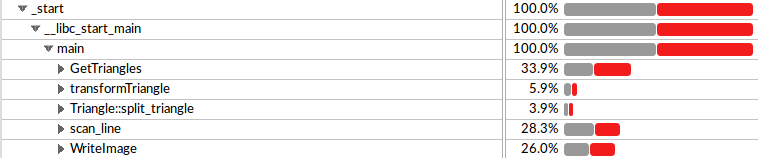
\includegraphics[width=1\textwidth]{./pictures/serial.png}
\label{serpro}
\caption{Performance results for Serial version}
\end{figure}

\subsubsection*{OpenMP}
Figure 2. provides the profiling results for OpenMP. With OpenMP we notices that it spends a lot of CPU time in OpenMP specific routines. this has our algorithm inside, but  OpenMP in general has a lot of overhead of thread scheduling.
\begin{figure}
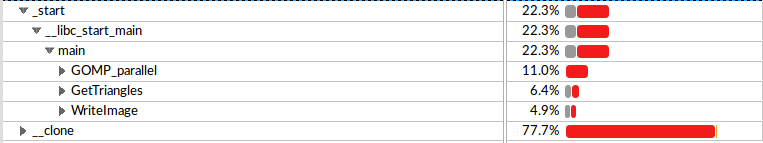
\includegraphics[width=1\textwidth]{./pictures/omp.png}
\label{omppro}
\caption{Performance results for OpenMP version}
\end{figure}

\subsubsection*{CilkPlus}
Figure 3. provides the profiling results for CilkPlus. With Cilk we got the best profiling results. The work done by the Cilk threads had very low overhead and gave pretty consistent results across multiple runs.
\begin{figure}
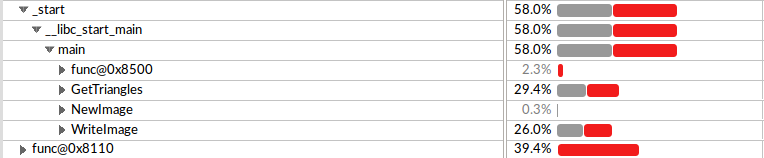
\includegraphics[width=1\textwidth]{./pictures/cilk.png}
\label{clkpro}
\caption{Performance results for Cilk version}
\end{figure}

\subsubsection*{TBB}
Figure 4. provides the profiling results for TBB. With TBB it's the same story as Cilk, However profiling tree was so huge that it is almost unreadble.
\begin{figure}
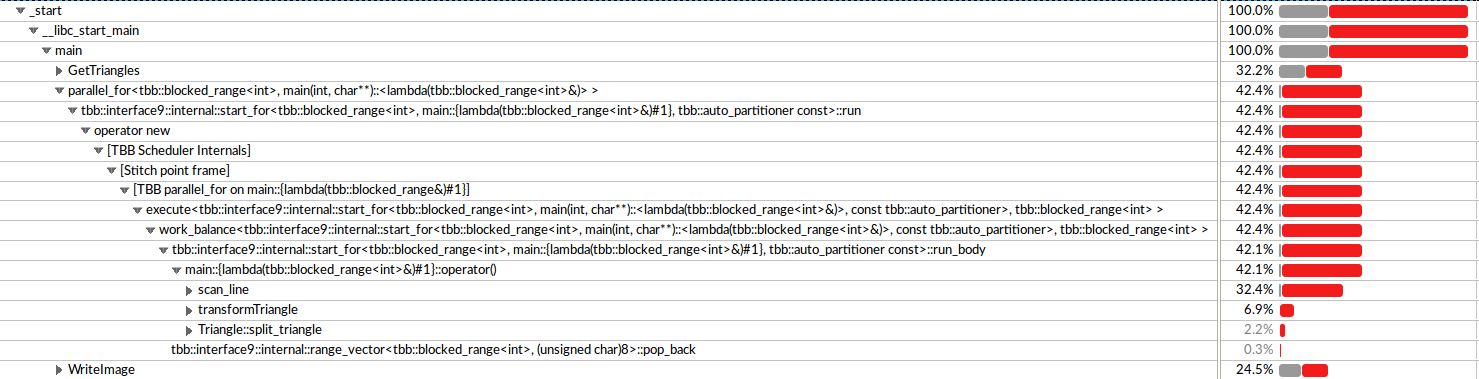
\includegraphics[width=1\textwidth]{./pictures/tbb.png}
\label{tbbpro}
\caption{Performance results for TBB version}
\end{figure}

